
\newcommand{\annotate}[1]{{\color{figloop!75!black} \mathsf{#1}}}

Fig.~\ref{fig:example} shows a fragment adapted from an industrial navigation component. Its \texttt{CheckCal} struct contains an array \texttt{pkv[10]}, its valid length \texttt{len}, and a sum field \texttt{chksum}. The caller \texttt{foo} invokes \texttt{CheckCalFun}, which sums the valid elements into \texttt{chksum}; an assertion in \texttt{foo} states the verification goal. This example raises three challenges:
\begin{itemize}
  \item \textbf{Loop reasoning:} The summation loop \texttt{for(; i<pIp->len; i++)} requires determining whether the initial state allows loop entry and, if it executes, establishing invariants that relate the partial sum to the processed array prefix.
  \item \textbf{Structs and pointers:} The procedures read and write struct fields through pointers, so specifications must account for aliasing and side effects: memory safety for dereferencing \texttt{pIp->pkv[i]}, the write effect on \texttt{pIp->chksum}, and frame properties for unchanged fields of \texttt{pIp}.
  \item \textbf{Inductive predicates:} Aggregate array properties such as sums are most naturally expressed with inductive predicates or logic functions; writing them in a verifier-friendly form and proving the resulting annotations remains a central challenge.
\end{itemize}

\begin{figure*}
    \centering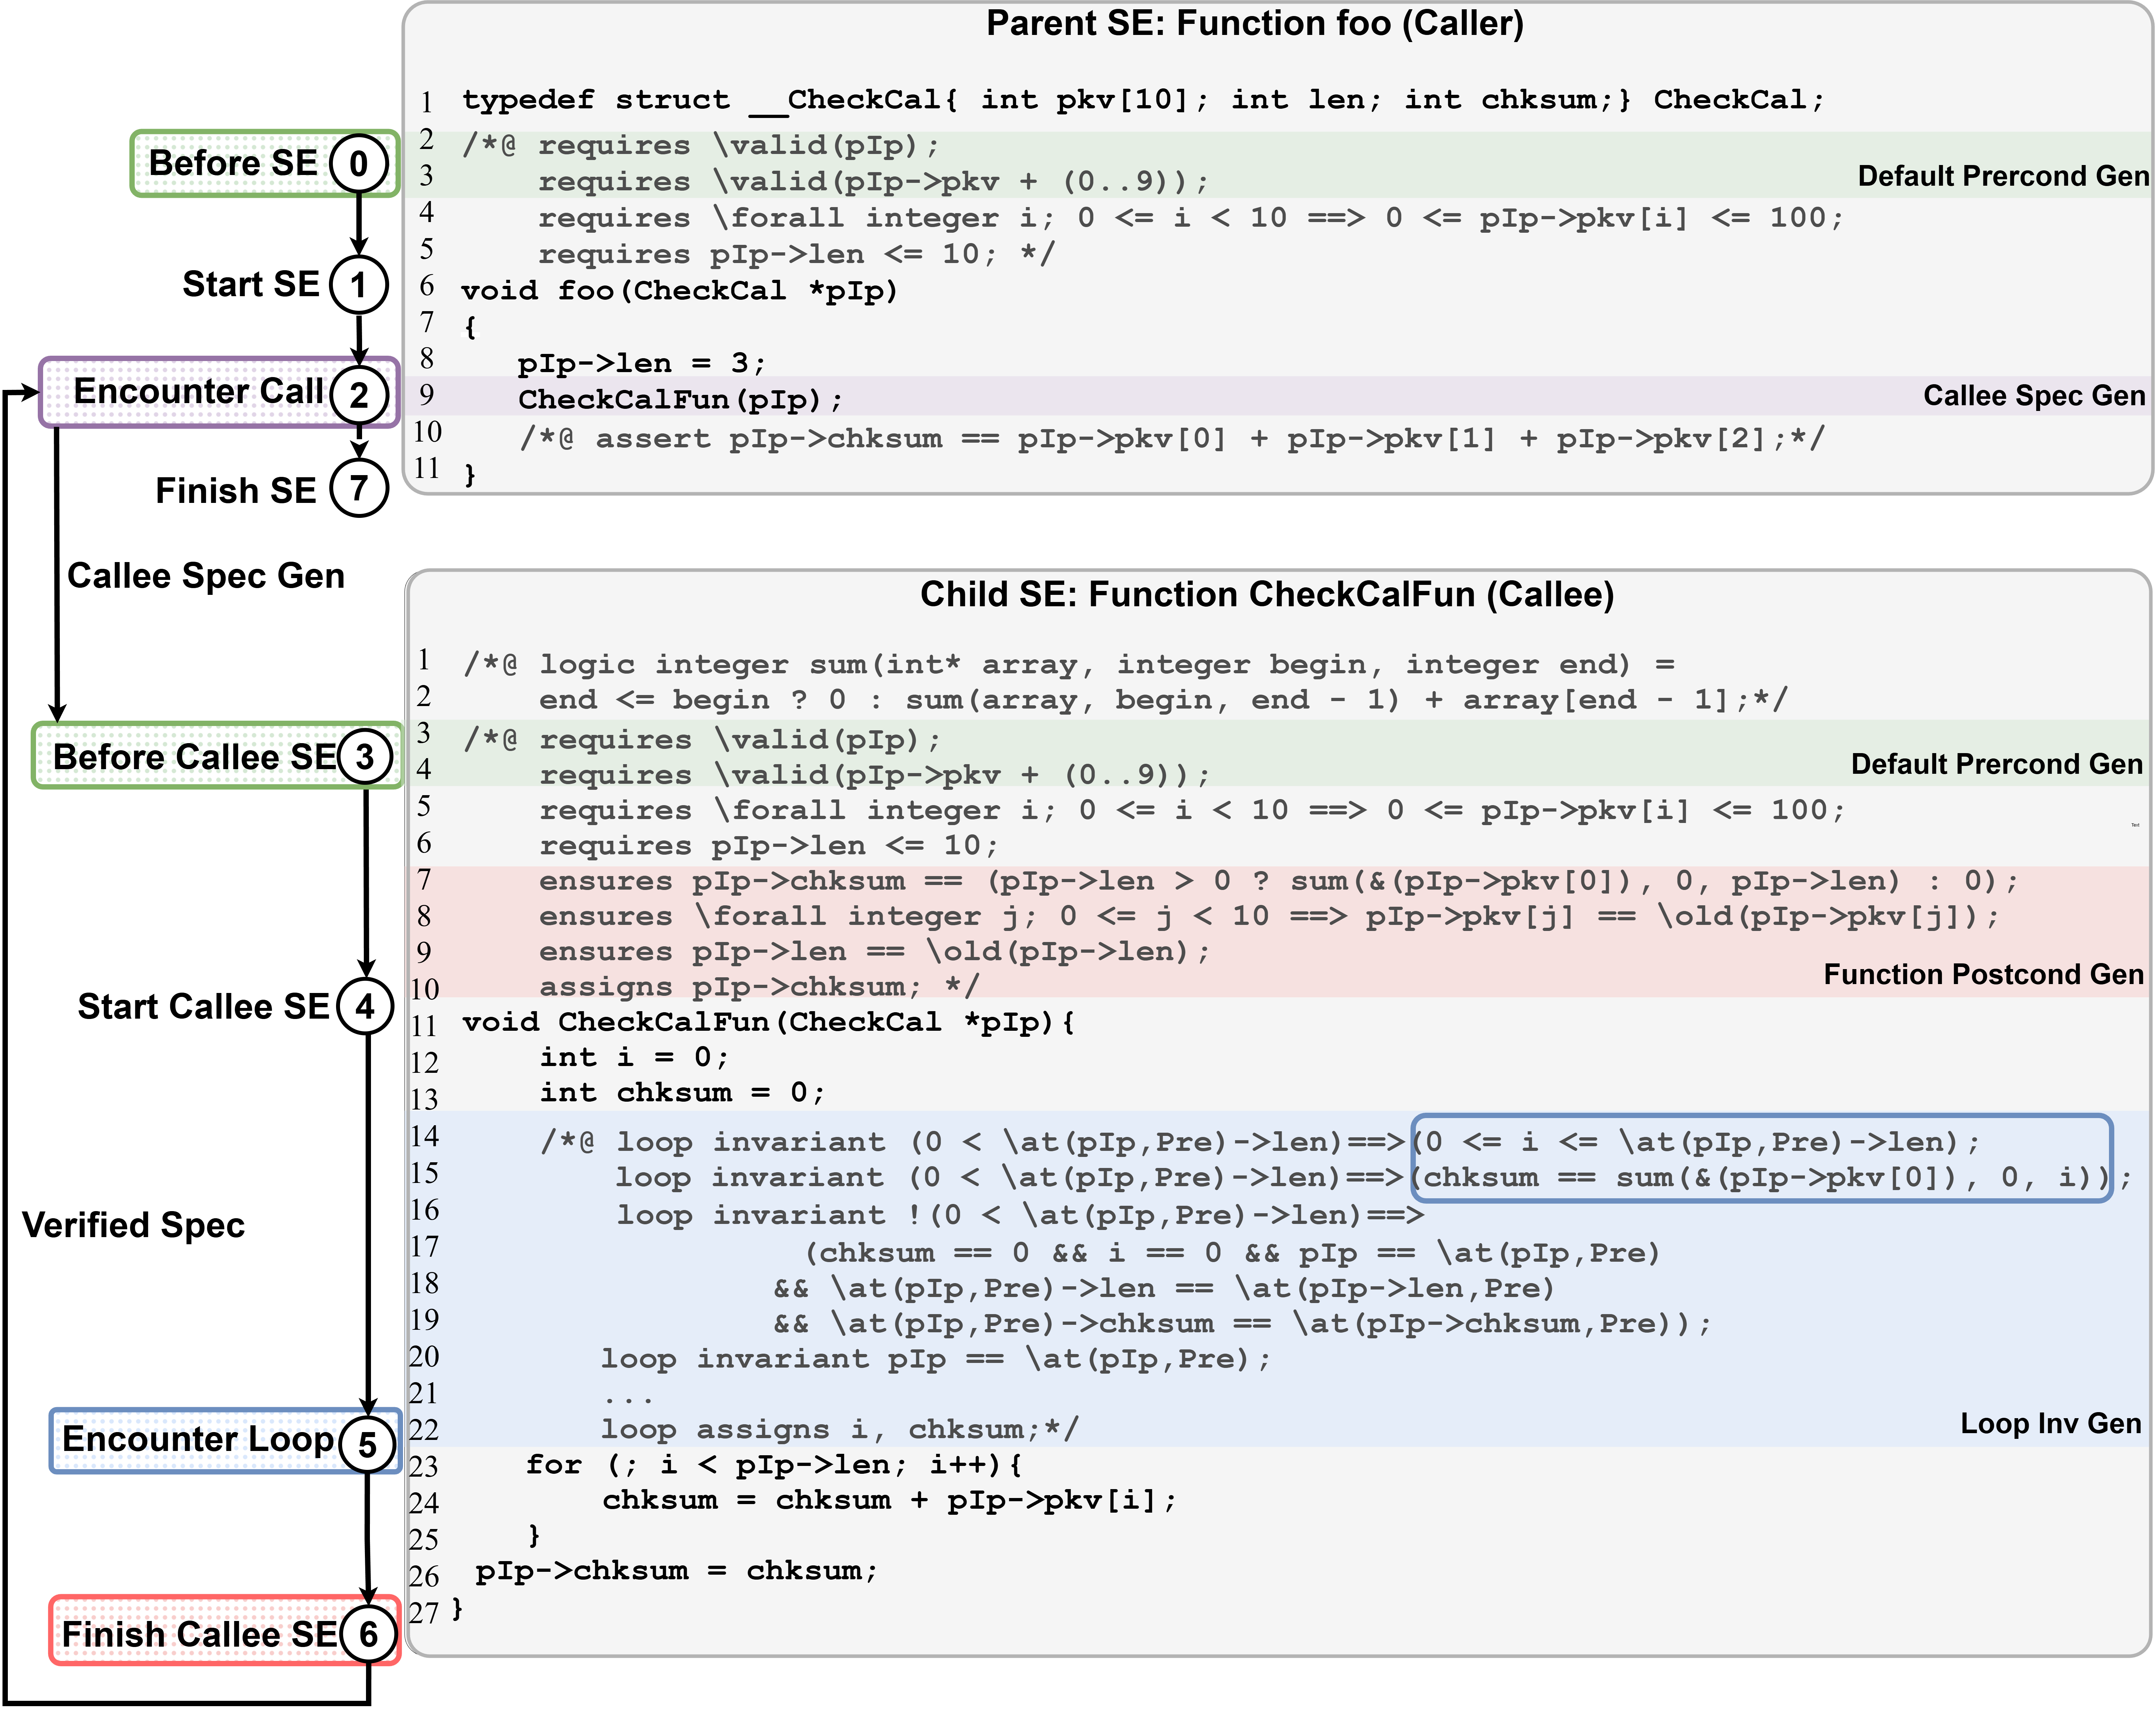
\includegraphics[width=0.72\textwidth]{images/example.png}
    \caption{Motivating Example}
    \label{fig:example}
\end{figure*}




Fig.~\ref{fig:example} annotates the example with ACSL \texttt{requires}, \texttt{ensures}, \texttt{loop invariant}, and \texttt{assert} clauses. \toolname\ generates the default preconditions, postconditions, and loop invariants; the assertion goal and additional \texttt{CheckCalFun} preconditions are supplied by the designers.


Before presenting our method, we attempted to generate the specification for this example using GPT-4o, Claude 3.7 Sonnet, and \autospec, given both the preconditions and the verification goal. The loop invariants they produced, shown below, were all found to be incorrect:

{\footnotesize
\[
\begin{array}{@{}l@{}}
\textsc{GPT-4o}\\
\texttt{loop invariant chksum == \textbackslash sum(0, i-1,}\\
\quad\texttt{\textbackslash lambda integer k; pIp->pkv[k]);}\\[3pt]
\textsc{Claude 3.7 Sonnet}\\
\texttt{loop invariant chksum ==}\\
\quad\texttt{\textbackslash sum(integer k = 0; k < i; pIp->pkv[k]);}\\[3pt]
\autospec\\
\texttt{loop invariant chksum == \textbackslash sum(0, i-1, pIp->pkv);}
\end{array}
\]
}

All three candidates include \texttt{0 <= i <= pIp->len} and a partial-sum relation, but omit the zero-iteration case (\texttt{pIp->len <= 0}); even a well-formed version therefore fails the base case. Explicitly prompting GPT-4o about this case did not produce a conditional invariant. Moreover, all three use \texttt{\textbackslash sum} without defining an ACSL logic function; their lambda, quantified-binder, and raw-pointer variants are rejected by Frama-C/WP.
 

 

 


 
